\usetikzlibrary{arrows.meta}
% id: 1996_shanghai_science_q7_optB; family: basic_conic
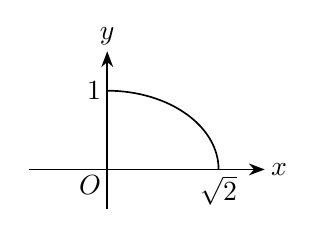
\begin{tikzpicture}[x=1cm,y=1cm,line width=.6pt,font=\normalsize,every node/.style={inner sep=0pt},>=Stealth]
\draw[->] (-1.0,0)--(2.0,0) node[right,inner sep=0pt,xshift=2pt] {$x$};
\draw[->] (0,-0.5)--(0,1.5) node[above,inner sep=0pt,yshift=2pt] {$y$};
\draw (1.4142135623730951,0) arc[start angle=0,end angle=90,x radius=1.4142135623730951cm,y radius=1cm];
\node[anchor=north east,inner sep=0pt,xshift=-2pt,yshift=-2pt] at (0,0) {$O$};
\node[anchor=east,inner sep=0pt,xshift=-2pt] at (0,1) {$1$};
\node[anchor=north,inner sep=0pt,yshift=-2pt] at (1.4142135623730951,0) {$\sqrt{2}$};
\end{tikzpicture}
